\newcommand{\notenumber}{2019-xx}
\newcommand{\notetitle}{\ac{bpcm} for intense electron beam driven plasmas in Nitrogen*}
\newcommand{\noteauthors}{P.~E.~Adamson}
\newcommand{\noteabstract}{A \acl{bpcm} is developed for intense electron
beam driven plasmas in Nitrogen.  This work is part of an effort to 
develop \acp{prm} for a DTRA- and NRL-funded effort to update ICEPIC and MEEC++ to
model \ac{sgemp}.}
%TODO: if new calcs, describe...
%TODO: if new data from literature, describe...
%TODO: If different decisions, describe...
%TODO: How will model be V&V'd?
\newcommand{\notesponsor}{DTRA/RD-NTE 6.2 program}

%TODO: use mhchem for all chemical species/equations
\documentclass[12pt]{article}
\usepackage{graphicx}
\usepackage{amsmath}
\usepackage{amssymb}
\usepackage{amscd}
\usepackage{siunitx}
\usepackage{bbm}
\usepackage{epstopdf}
\DeclareGraphicsRule{.tif}{png}{.png}{`convert #1 `dirname #1`/`basename #1 .tif`.png}
\usepackage{color,soul}
\usepackage{rotating}
\usepackage{multirow}
\usepackage[htt]{hyphenat}
\usepackage[version=4]{mhchem}
\usepackage{subfigure}
\usepackage{dcolumn}
\usepackage{wrapfig}
\usepackage[nolist,nohyperlinks]{acronym}
\usepackage{array}
%\usepackage{parskip}
%\parskip=1em
\usepackage{verbatimbox}
\usepackage{listings}

\newcommand*{\restrictlinewidthbox}[1]{%
  \begingroup
    \sbox0{#1}%
    \ifdim\wd0>\linewidth
      \resizebox{\linewidth}{!}{\copy0}%
    \else
      \copy0 %
    \fi
  \endgroup
}

\newcolumntype{d}[1]{D{.}{.}{#1}}
\newcommand\mc[1]{\multicolumn{1}{c}{#1}}
\newcommand{\vect}[1]{\boldsymbol{#1}}

%\usepackage{tikz,pgfplots}
%\pgfplotsset{compat=newest} 
%\pgfplotsset{plot coordinates/math parser=false}

% for better list... used for custom title page
\usepackage{enumitem}

%\usepackage{pgf}
%\usepackage{pgffor}
%\usepgflibrary{plothandlers}

%\usepgfplotslibrary{external} 
%\tikzexternalize% activate externalization!

% use this to remake a particular plot...
%\tikzset{external/remake next}

%use this to remake all
%\tikzset{external/force remake}

%\tikzsetexternalprefix{figures/}

%% Fonts %%
\usepackage{microtype}

\usepackage[T1]{fontenc}
\usepackage{textcomp}

% Times New Roman
\usepackage{mathptmx}

% this stuff is to make the section headings look like phys plasmas
\usepackage[scaled=.92]{helvet}
%\usepackage{helvet}

% NB, use citenum to get inline citation (not superscript)

\usepackage[colorlinks=true,
		citecolor=blue,
		linkcolor=blue,
		anchorcolor=blue,
		filecolor=blue,
		menucolor=blue,
		runcolor=blue,
		urlcolor=blue,
		unicode
		]{hyperref}
\usepackage[all]{hypcap}

%
\usepackage{geometry}
\geometry{margin=1in}

\usepackage{sectsty}  
%\sectionfont{\normalfont\sffamily\large\underline\bfseries\color{orange}}
%\sectionfont{\normalfont\sffamily\large\bfseries\color{orange}\sectionrule{0pt}{??0pt}{-4pt}{1pt}}
%\sectionfont{\normalfont\sffamily\large\bfseries\sectionrule{3ex}{3pt}{-1ex}{1pt}}
\sectionfont{\normalfont\sffamily\large\bfseries}
\subsectionfont{\normalfont\sffamily\normalsize\bfseries}

\newcommand{\mycomment}[1]{}
\newcommand{\tbd}{\textcolor{red}{\textbf{\hl{TBD}}}}

% set noindents for entire document
\setlength\parindent{0pt}
%\setlength{\parskip}{1em}

\newcolumntype{P}[1]{>{\centering\arraybackslash}p{#1}}

%%%%%%%%%%%%%%%%%%%%%%%%%%%%%%%%%%%%%%%%%%%%
%% BEGIN DOCUMENT
%%%%%%%%%%%%%%%%%%%%%%%%%%%%%%%%%%%%%%%%%%%%
\begin{document}
/Users/adamson/projects/latex/acronyms.tex
\graphicspath{{./fig/}}
\begin{titlepage}

\rmfamily
\begin{center}\sffamily\bfseries
PULSED POWER PHYSICS TECHNOTE NO. \notenumber{}\\
{~}
\end{center}

\begin{description}[leftmargin=8em,style=nextline,font=\sffamily\bfseries ]
\item[TITLE:]{\bfseries 
\notetitle{}
}
\item[AUTHORS:]{ \noteauthors{}\\
{\itshape Code 6770, Plasma Physics Division, Naval Research Laboratory}}
\item[DATE:]\today
\item[ABSTRACT:] 
\noteabstract{}
\end{description}

\vfill

{\small
\noindent THIS REPORT REPRESENTS UNPUBLISHED INTERNAL WORKING DOCUMENTS AND SHOULD NOT BE REFERENCED OR DISTRIBUTED WITHOUT THE AUTHORS' CONSENT

{~}

\noindent * Work supported by \notesponsor{}. 
}
\end{titlepage}

\pagestyle{myheadings}



\markright{\hfill \color{red}\sf DRAFT VERSION DO NOT CIRCULATE \hfill}

\newcommand{\etal}{\textit{et. al.}}
\newcommand{\bpcmn}{$\text{bPCM}_\text{N}$}

\section{Introduction}

\begin{table}
		\caption{N species available in the \bpcmn{} are those tracked by Angus, \etal{} in ref~\cite{angus2016}. All of the 
		molecular-excitation energies listed are with respect to the ground neutral molecular state and
		similarly for the atomic species with charge state $Z\ge1$. The energies listed for the atomic ion species
		with $Z>1$ are with respect to the ground electronic state of the $Z-1$ charge state.} \label{tab:bl_species}
		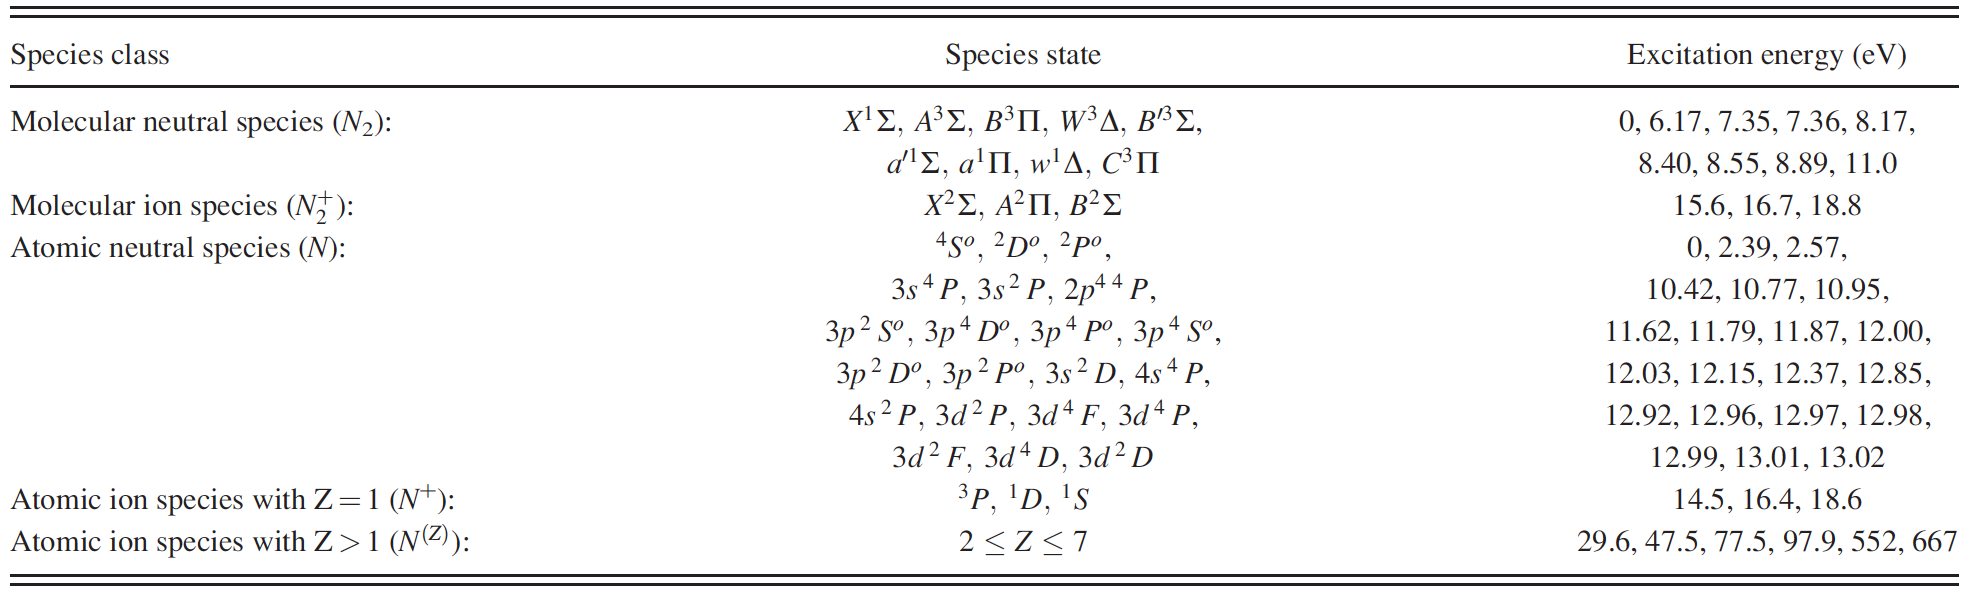
\includegraphics[width=\textwidth]{bl_species.eps}
\end{table}

\begin{wraptable}{r}{6cm}
		\vspace{-50pt}
		\caption{Spectroscopic target states of atomic nitrogen for neutral atom excitation, 
		ionization, and elastic scattering cross sections. The indices in the first column of the table are used to
		catalog the raw \ac{bsr} and LxCat format data files as described in Table~\ref{tab:N_filenames}.} \label{tab:N_states}
		\centering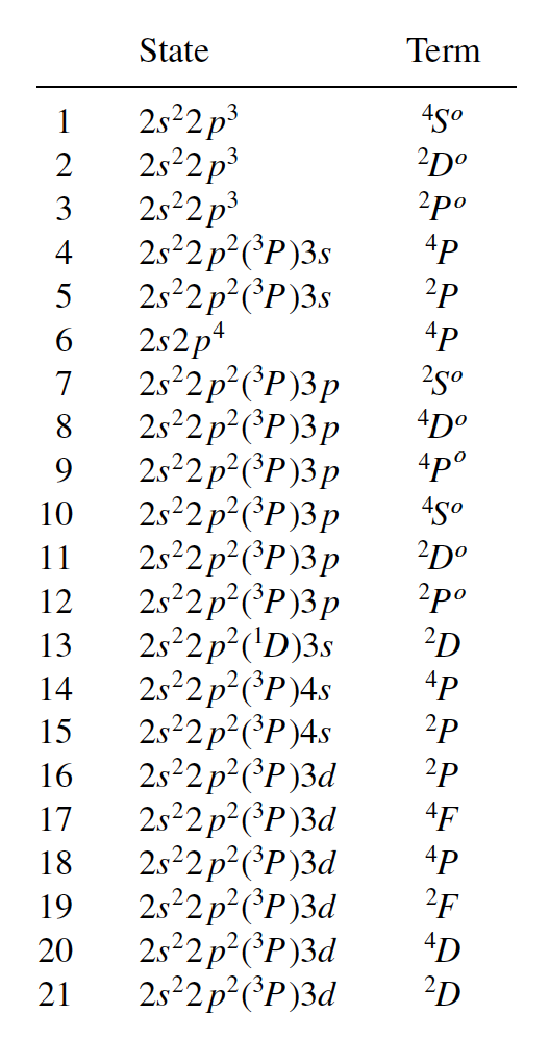
\includegraphics[width=0.3\textwidth]{N_states.eps}
		\vspace{-50pt}
\end{wraptable}

Species available in the \acl{bpcm} for Nitrogen (\bpcmn) are those tracked by Angus, \etal{} in ref~\cite{angus2016}, 
as shown in Table~\ref{tab:bl_species}.
%TODO: if new calcs, describe...
%TODO: if new data from literature, describe...
%TODO: If different decisions, describe...
%TODO: How will model be V&V'd?


\section{Molecular neutral species (\ce{N2})}

\begin{table}
		\caption{\ce{N2} excited states}
		\begin{tabular}{c c}
				\hline\hline
				Index & Symbol \\
				 & \multicolumn{6}{c}{Electron configuration} & \\ \cline{2-7}
Index & 2\ce{\sigma_u} & 1\ce{\pi_u} & 3\ce{\sigma_g} & 1\ce{\pi_g} & 3\ce{\sigma_u} & 3\ce{\sigma_g} & Term\\
\hline
1  & 2 & 4 & 2 & 0 & 0 & 0 & X ${}^1\Sigma_g^+$ \\
2  & 2 & 3 & 2 & 1 & 0 & 0 & A ${}^3\Sigma_u^+$ \\
3  & 2 & 4 & 1 & 1 & 0 & 0 & B ${}^3\Pi_g$ \\
4  & 2 & 3 & 2 & 1 & 0 & 0 & W ${}^3\Delta_u$ \\
5  & 2 & 3 & 2 & 1 & 0 & 0 & $\text{B}^\prime\;{}^3\Sigma_u^-$ \\
6  & 2 & 3 & 2 & 1 & 0 & 0 & $\text{a}^\prime\;{}^1\Sigma_u^-$ \\
7  & 2 & 4 & 1 & 1 & 0 & 0 & $\text{a}\;{}^1\Pi_g$ \\
8  & 2 & 3 & 2 & 1 & 0 & 0 & w ${}^1\Delta_u$ \\
9  & 1 & 4 & 2 & 1 & 0 & 0 & C ${}^3\Pi_u$ \\
10 & 2 & 4 & 1 & 0 & 0 & 1 & E ${}^3\Sigma_g^+$ \\ 
11 & & & & & & & $\text{a}^{\prime\prime}\;{}^1\Sigma_g^+$ \\  



				\hline\hline
		\end{tabular}
\end{table}




\section{Molecular ion species (\ce{N2+})}
\tbd


\section{Neutral N Atom}

The neutral N atomic species followed in \bpcmn{} include
the ground state $\ce{2s^2 2p^3}\;\ce{^4S^o}$, the two low lying meta stable states
that share the same electron configuration as the ground state
$(1s^22s^22p^3)\; N(\ce{^2D^o}, \ce{^2Po})$, and the first 18 optically allowed 
excited states.  These electronic states and corresponding term symbols
are listed in Table~\ref{tab:N_states}. 

\subsection{Electron-Impact Excitation Cross Sections}

For \bpcmn{}, electron-impact excitation
%, elastic scattering, and electron-impact ionization 
cross sections between electronic 
states of neutral
atomic nitrogen listed in Table~\ref{tab:N_states} are taken from \ac{bsr}
calculations by Wang~et~al.\cite{wang2014} 
Table~\ref{tab:N_filenames} describes the file naming schemes and locations of LxCat and raw (\ac{bsr} output)
format data files for cross sections from ref~\cite{wang2014}, including elastic scattering and electron-impact 
ionization cross sections which will be described below. \\

Some details of the BSR model from ref~\cite{wang2014}:
\begin{itemize}
		\item the configuration expansions for each atomic target state
				contained up to 250 configurations
		\item the number of pseudostates used to describe ionization processes
				was limited by a relatively small box size of radius $30 a_0$, thus 
				restricting the number of spectroscopic target states that could be
				accurately modeled to those listed in Table~\ref{tab:N_states}
		\item the \ac{cc} expansion includes 690\footnote{note the discrepancy
				between the total size of the expansion (690) and the sum of the bound and continuum
				state quantities (56+644=700)} states of atomic
				nitrogen, with 56 states representing the bound spectrum
				and the remaining 644 representing the target continuum
				and some core-excited autoionizing states
		\item all doublet and quartet target states with total electronic orbital
				angular momentum $L = 0–4$ are included
		\item the continuum pseudostates cover the energy regime up to 50~eV
				above the ionization limit
		\item the maximum interval in the B-spline grid is $0.65 a_0$, which is
				sufficient to cover electron scattering energies up to $200~eV$
		\item the collision model contained up to 1704 scattering channels, leading to generalized eigenvalue
				problems with matrix dimensions up to 120,000 in the \bspline{} basis 
		\item partial waves for total orbital angular momenta $L\le25$ were computed numerically
				resulting in 156 partial waves when spin and parity are taken into account
\end{itemize}

In order to assess the accuracy and completeness of the BSR results of ref~\cite{wang2014}, we plan to reproduce them with the \ac{ukrmol+}
				\ac{bto}/\ac{gto} method while varying the following parameters: 
				\begin{itemize}
						\item quantum mechanical method for target wave function (\ac{hf}, 
								\ac{cas}-\ac{ci}, \ac{fc}-\ac{fci}, \ac{fci}) including the number of configurations in included in the \ac{ci},
						\item basis set size and type in target wave function,
						\item custom even-tempered versus off-the-shelf basis sets in target
								wave function, 
						\item extent of the reduced radial range and target-continuum transition,
						\item continuum \ac{bto}/\ac{gto} basis size and parameters, and
						\item \bspline{} grid interval
				\end{itemize} 

\begin{sidewaystable}
		\caption{Filename structure for example neutral N atom electron-impact excitation, 
		elastic scattering, and electron-impact ionization cross sections stored in LxCat and raw (\ac{bsr} output)
		format. The first and second numbers used in  
		the filenames correspond to the indices from the first column of Table~\ref{tab:N_states} for the 
		\ac{lhs} and \ac{rhs} N atom species, respectively. Raw data from \ac{bsr} calculations are stored in
		the \texttt{n\_bsr/N\_2014\_archive} folder. Data files in LxCat format are stored in the
		\texttt{n\_bsr/lxcat} folder.} \label{tab:N_filenames}
		\centering
		\begin{tabular}{l r c l P{1cm} P{1cm} c c}
				\hline\hline
				Process & & & & LHS Index & RHS Index & Format & Filename \\
				\hline
				\multirow{2}{*}{\parbox{2cm}{Electron-Impact Excitation}} & \rule{0pt}{1em}$e^- + N[(2s^22p^3)\; ^4S^o]$ & $\rightarrow$ & $e^- +N[(2s^22p^3)\; ^2D^o]$ & 1 & 2 & LxCat & \texttt{tr\_001\_002\_lxcat} \\
				&                               & &                                            &   &   & BSR & \texttt{tr\_001\_002}        \\[.5em]
				& $e^- + N[(2s^22p^3)\; ^2D^o]$ & $\rightarrow$ & $e^- +N[(2s2p^4)\; ^4P]$     & 2 & 6 & LxCat & \texttt{tr\_002\_006\_lxcat} \\
				&                               & &                                            &   &   & BSR & \texttt{tr\_002\_006}        \\
				\hline
				\multirow{2}{*}{\parbox{2cm}{Elastic Scattering}}& \rule{0pt}{1em}$e^- + N[(2s^22p^3)\; ^4S^o]$ &&& 1 & 1 & LxCat & \texttt{tr\_001\_001\_lxcat} \\
				&                               & & &   &   & BSR   & \texttt{tr\_001\_001}        \\[.5em]
				& $e^- + N[(2s^22p^3)\; ^2D^o]$ & & & 2 & 2 & LxCat & \texttt{tr\_002\_002\_lxcat} \\
				&                               & & &   &   & BSR   & \texttt{tr\_002\_002}        \\
				\hline
				\multirow{2}{*}{\parbox{2cm}{Electron-Impact Ionization}} & \rule{0pt}{1em}$e^- + N[(2s^22p^3)\; ^4S^o]$ & $\rightarrow$ & $e^- + e^- + N[(2s^22p^3)\; ^4S^o]^+$ & 1 & N/A & LxCat & \texttt{ion\_001\_lxcat} \\
				&                               & & &  &  & BSR & \texttt{ion\_001}        \\[.5em]
				& $e^- + N[(2s^22p^3)\; ^2D^o]$ &$\rightarrow$ &$e^- + e^- + N[(2s^22p^3)\; ^2D^o]^+$ & 2 & N/A & LxCat            & \texttt{ion\_002\_lxcat} \\
				&                               & & &  & & BSR & \texttt{ion\_002}        \\
				\hline\hline
		\end{tabular}
\end{sidewaystable}

\subsection{Electron-Impact Ionization} 
\tbd

\subsection{Elastic Scattering}
\tbd

\section{Singly-Ionized Nitrogen Ion}

For the singly ionized atomic nitrogen ion species, the states
considered are the ground state $N^+\;(^3P)$ and the two low–lying
meta stable states that share the same electron configuration as
the ground state $(1s^22s^22p^2)\; N^+\; (^1D,\; ^1S)$. 

\subsection{Electron-Impact Excitation Cross Sections}
Cross sections for the two processes considered,
\begin{align}
		\ce{e-} + \ce{N}\left[(2s^22p^2)\; \ce{^3P}\right]^+ & \rightarrow \ce{e-} +\ce{N}[(2s^22p^2)\; \ce{^1D}]^+\\
		\ce{e-} + \ce{N}\left[(2s^22p^2)\; \ce{^3P}\right]^+ & \rightarrow \ce{e-} +\ce{N}[(2s^22p^2)\; \ce{^1S}]^+
\end{align}
are calculated using the approach from references \cite{henry1969} and \cite{taylor1988}:
\begin{equation}
		\sigma_j = \left[\left(1.197\times 10^{-15}\right)/g_i E\right]\Omega(1,j)
\end{equation}
where $g_i$ is the initial state statistical weight ($g_i = 9$) and $\Omega(1,j)$
is the collision strength for the final state. Although the collision strengths have
energy dependence as shown in Figure~\ref{fig:cs_Nii}, we will use the 
constant values given in Table~\ref{tab:cs_Nii} consistent with the approach in ref~\cite{henry1969}.
The relevant cross sections are stored in LxCat format in the files listed in 
Table~\ref{tab:np_excitation_files}.
\textit{Note: ref~\cite{taylor1988} also provides approaches for computing electron-impact
excitation cross sections for six optically allowed $N^+$ transitions to triplet
states as well as excitations to Rydberg-states that are not included in this baseline
plasma chemistry model.}

Improvements: \tbd

%%%%%%%%%%%%%%%%%%%%%%%%%%%%%%%%%%%%%%%%%%%%%%%%%%%%%%%%%%%%%%%%%%%%%%%%%%%%%%%%%%
% We will ignore energy dependence as is done in ref~\cite{henry1969}
%
%determined by digitizing the relevant plots in ref~\cite{henry1969}, shown in
%The data were digitized using the Engauge Digitizer app, and 
%$\Omega(1,2)$, $\Omega(1,3)$, and $\Omega(2,3)$ are stored in
%\texttt{np\_henry/collision\_strength\_Nii\_001\_002.csv} and
%\texttt{np\_henry/collision\_strength\_Nii\_001\_003.csv}, respectively.
%\texttt{np\_henry/collision\_strength\_Nii\_002\_003.csv}, respectively.  
%%%%%%%%%%%%%%%%%%%%%%%%%%%%%%%%%%%%%%%%%%%%%%%%%%%%%%%%%%%%%%%%%%%%%%%%%%%%%%%%%%

\begin{figure}
		\subfigure[$\Omega(1,2)$]{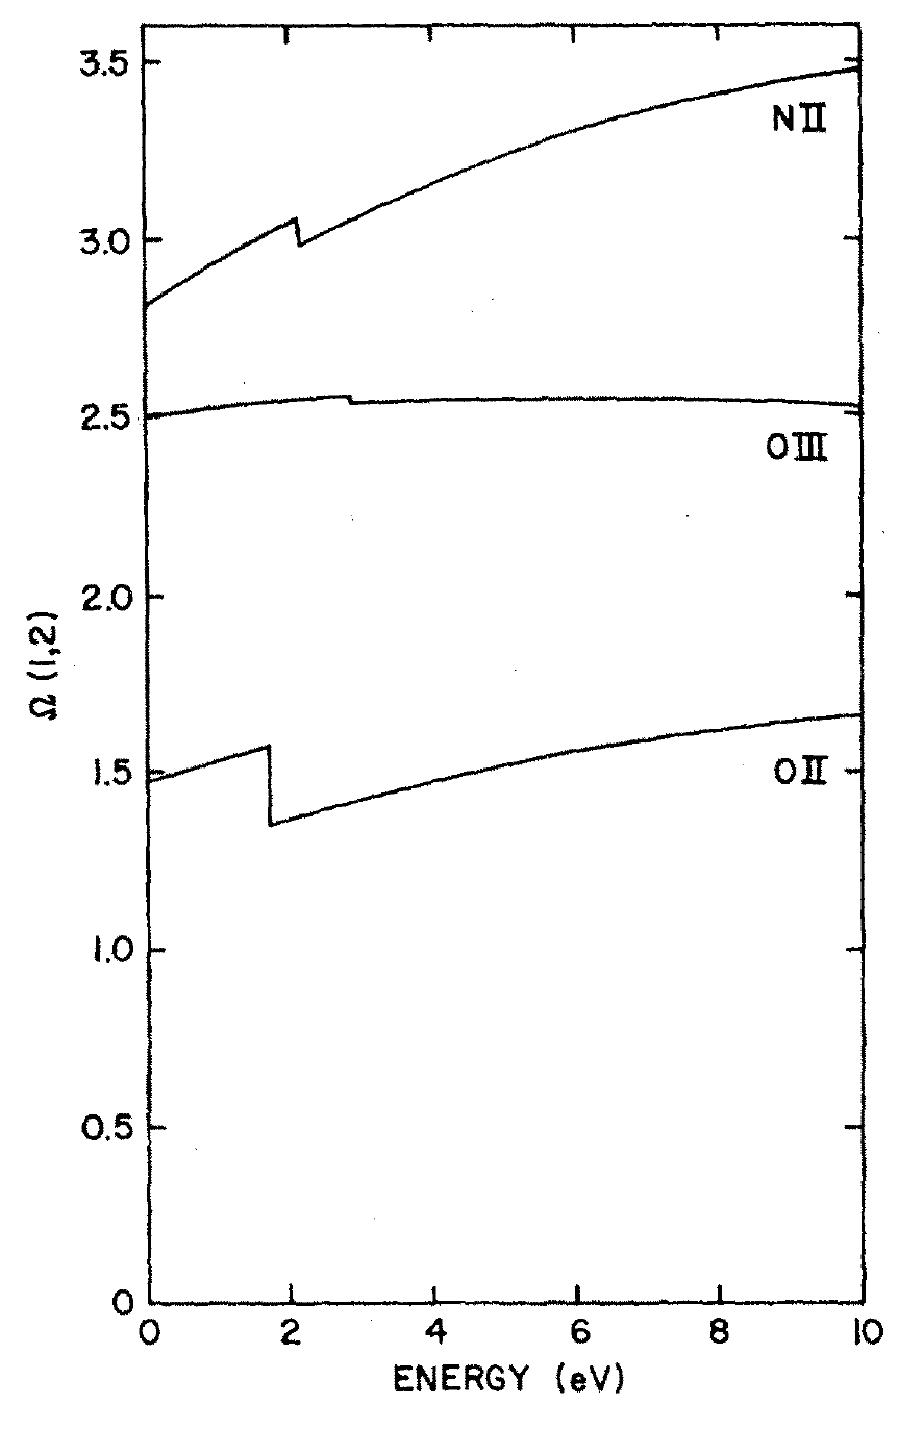
\includegraphics[width=0.4\textwidth]{cs_Nii_1_2.eps}}
		\subfigure[$\Omega(1,3)$]{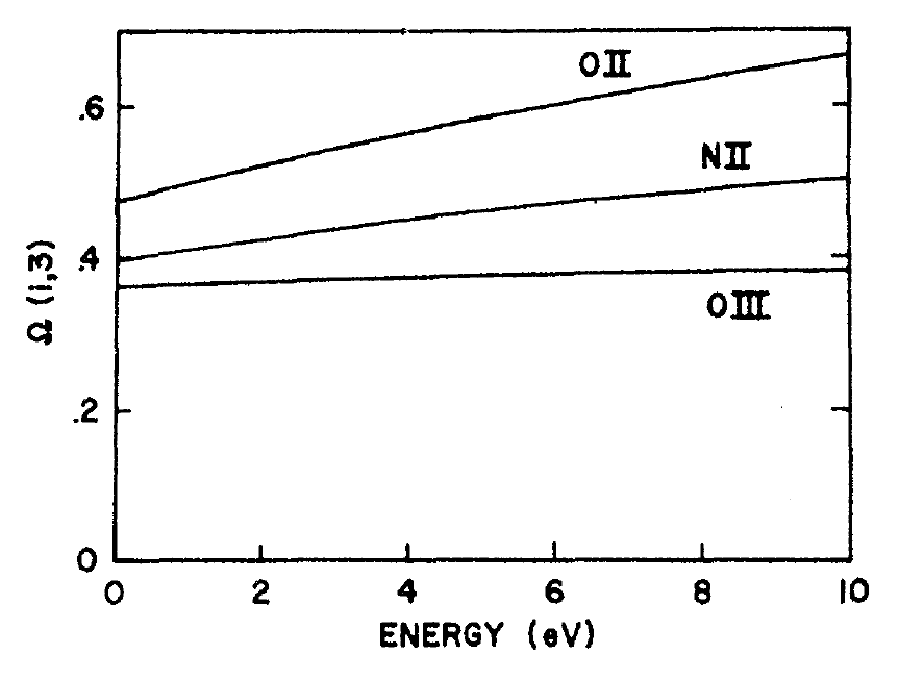
\includegraphics[width=0.4\textwidth]{cs_Nii_1_3.eps}}
		%		\subfigure[$\Omega(2,3)$]{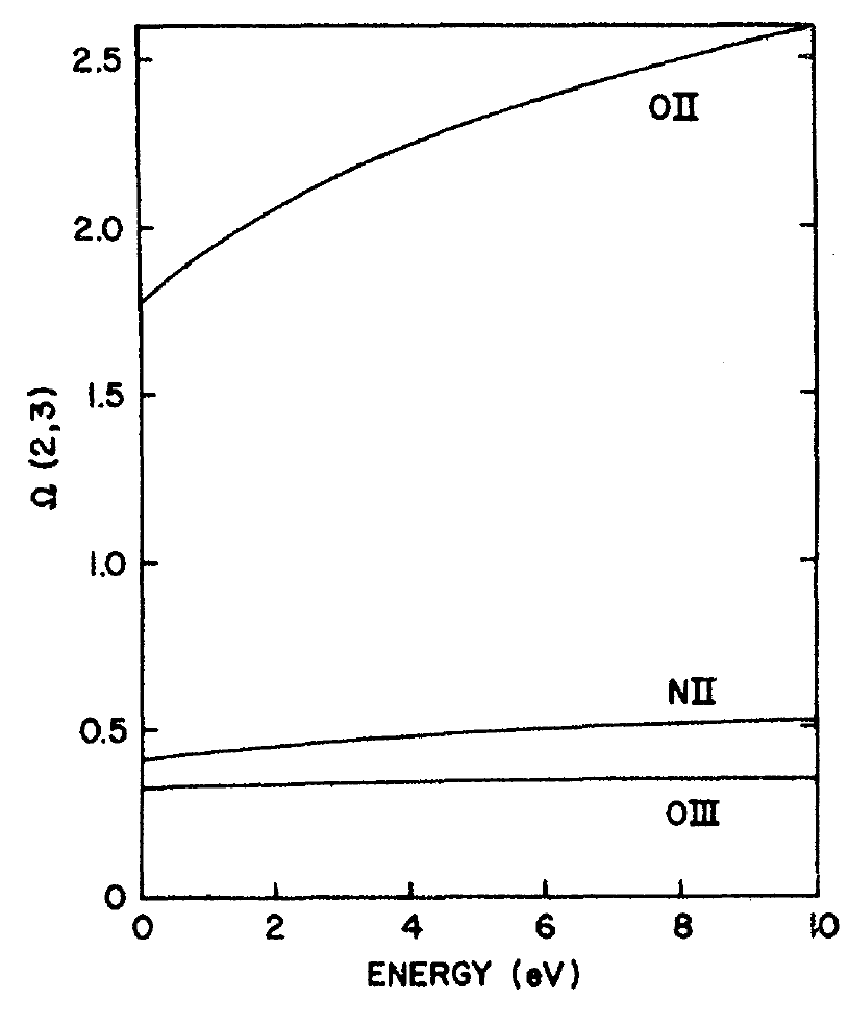
\includegraphics[width=0.3\textwidth]{cs_Nii_2_3.eps}}
		%
		\caption{Energy variation of collision strengths
		for electrons incident on \ce{N+}, \ce{O+}, and \ce{O++} ions from
		ref~\cite{henry1969}.}\label{fig:cs_Nii}
\end{figure}

\begin{table}
		\caption{Collision strengths $\Omega(i,j)$.}\label{tab:cs_Nii}
		\centering
		\begin{tabular}{c c d{1.3}}
				\hline\hline
				$i$ & $j$ & \mc{$\Omega(i,j)$} \\
				\hline
				\rule{0pt}{1em}\ce{^3P} & \ce{^1D} & 2.98 \\
				\ce{^3P} & \ce{^1S} & 0.395 \\
				\ce{^1D} & \ce{^1S} & 0.410 \\
				\hline\hline
		\end{tabular}
\end{table}

\begin{table}
		\caption{Nitrogen ion electron-impact excitation cross section files.}\label{tab:np_excitation_files}
		\centering
		\begin{tabular}{l l}
				\hline\hline
				Process & Cross Section File\\
				\hline
				$\ce{e-} + \ce{N}\left[(2s^22p^2)\; \ce{^3P}\right]^+ \rightarrow \ce{e-} +\ce{N}[(2s^22p^2)\; \ce{^1D}]^+$ & \texttt{np\_henry/tr\_001\_002\_lxcat}\\
				$\ce{e-} + \ce{N}\left[(2s^22p^2)\; \ce{^3P}\right]^+ \rightarrow \ce{e-} +\ce{N}[(2s^22p^2)\; \ce{^1S}]^+$ & \texttt{np\_henry/tr\_001\_003\_lxcat}\\
				\hline\hline
		\end{tabular}
\end{table}

\subsection{Electron-Impact Ionization Cross Sections} 
\tbd

\subsection{Elastic Scattering Cross Sections}
\tbd

\section{Ionized Atomic Nitrogen ($Z>1$)}
The ground electronic
states of ionized atomic nitrogen with charge state $Z>1$
are also contained in the model. None of the $Z>1$ species
have low–lying electronic levels that share the same ground–
state–electron configuration.

\subsection{Electron-Impact Excitation Cross Sections} 
\tbd

\subsection{Electron-Impact Ionization Cross Sections} 
\tbd

\subsection{Elastic Scattering Cross Sections}
\tbd


\section{Summary}

\begin{sidewaystable}
		\caption{Neutral N atom plasma chemistry model--baseline and preliminary improvement approach.}
		\centering
		\begin{tabular}{ p{4cm} p{5cm} p{12cm} }
				\hline\hline
				Process & Baseline & Preliminary Improvement Approach \\ \hline
				Electron-Impact Excitation & \ac{bsr}\cite{wang2014} & 
				Reproduce ref~\cite{wang2014} \ac{bsr} results with the \ac{ukrmol+}
				\ac{bto}/\ac{gto} method;
				explore impact of varying: 
				\begin{itemize}
						\item quantum mechanical method for target wave function (\ac{hf}, 
								\ac{cas}-\ac{ci}, \ac{fc}-\ac{fci}, \ac{fci}) including the number of configurations in included in the \ac{ci},
						\item basis set size and type in target wave function,
						\item custom even-tempered versus off-the-shelf basis sets in target
								wave function, 
						\item extent of the reduced radial range and target-continuum transition,
						\item continuum \ac{bto}/\ac{gto} basis size and parameters, and
						\item \bspline{} grid interval
				\end{itemize} \\
				Electron-Impact Ionization & &  \\
				Elastic Scattering & &  \\
				\hline
		\end{tabular}
\end{sidewaystable}

\begin{sidewaystable}
		\caption{Singly-ionized N atom plasma chemistry model--baseline and preliminary improvement approach.}
		\centering
		\begin{tabular}{ p{5cm} p{8cm} p{8cm} }
				\hline\hline
				Electron-Impact Excitation &  & \\
				Electron-Impact Ionization &  & \\
				Elastic Scattering & &  \\
				\hline
		\end{tabular}
\end{sidewaystable}

\begin{sidewaystable}
		\caption{Ionized N atom ($Z>1$) plasma chemistry model--baseline and preliminary improvement approach.}
		\centering
		\begin{tabular}{ p{5cm} p{8cm} p{8cm} }
				\hline\hline
				Electron-Impact Excitation &  & \\
				Electron-Impact Ionization & & \\
				Elastic Scattering & & \\
				\hline
		\end{tabular}
\end{sidewaystable}

\clearpage 

\appendix

\section{\rmat{} Method Considerations}
In \rmat{} methods, 
the scattering problem is divided into inner
and outer regions separated by a
sphere of radius $r=a$ upon which the energy-dependent \rmat
is constructed. In the inner region, quantum chemistry
methods, such as \ac{hf} and post-\ac{hf} methods found in
codes such as \ac{gamess}\cite{gamess1993} and Gaussian\cite{g16}, 
are used to produce full scattering energy-independent
wavefunctions for the target molecule and for the target
molecule plus the scattering electron. The form of the inner
region wavefunction is

\begin{equation}
		\Psi_k = \hat{A}\sum_{i,j} c_{ijk} \Phi_i^N \eta_j + \sum_m b_{mk} X_m^{N+1} \label{eq:inner}
\end{equation}

The first of the two terms in equation~\ref{eq:inner} is a sum over
products of the target wavefunctions, $\Phi_i^N$, and
the continuum orbitals, $\eta_j$, where $c_{ijk}$ is the coefficient for the
$i$th, $j$th, $k$th term. $N$ labels the target wavefunction ($N$ electrons in the target atom).
The second term, called the $L^2$ term, is
necessary to describe polarisation/correlation and resonance
formation. This involves forming a wavefunction of the target
molecule plus the scattering electron (hence the $N+1$ label) using occupied and
virtual target orbitals, the $X_m^{N+1}$,
where $b_{mk}$ is the coefficient for the $m$th, $k$th term.
A crucial assumption applied when selecting the target
model is that the target wavefunction is entirely contained
within the \rmat{} sphere. In the outer region, the \rmat
is propagated to a large radius (typically on the order of 100~$a_0$), 
then used to calculate $K$- and $T$-matrices which give scattering quantities
such as eigenphases, cross-sections, and resonances.\\

The quality of \rmat{} calculations are highly dependent on several factors:
\begin{enumerate}
		\item the amount of electron correlation captured by the quantum chemistry
				treatment used to compute the target wavefunction, $\Psi$
		\item the size, nature, and quality of the atomic basis set used in \#1 (also
				affects amount of electron correlation included in the model)
		\item inclusion of polarization/correlation and excited states in the 
				scattering model
		\item number of continuum basis functions used to represent the continuum
				orbitals, $X$
\end{enumerate}

\subsection{Target model}

The simplest \textit{ab initio} quantum chemistry
treatment in common usage is the \ac{hf} method,
in which electrons only interact with the mean averaged field
of other electrons and nuclei. The corresponding \ac{hf} wavefunction
is represented by a single configuration. On the other
end of the accuracy scale is the \ac{fci}
method, which includes all possible electron configurations
constructed from all available \acp{mo}
subject only to the constraints of the Pauli Principle and total
symmetry, giving the best possible wavefunctions for a given
basis set. Intermediate between these is
\ac{cas}-\ac{ci} where only
a subset of the available HF \acp{mo} are in the ``active space'' 
of the FCI method. A
special variant of the CAS-CI method is the \ac{fc}-FCI
model where the core \acp{mo} are always
doubly occupied and the remaining electrons are active in all
the other orbitals. \\

%TODO: describe FC-FCI for N and N2
%For BeH the FC-FCI approximation corresponds
%to freezing the two 1s electrons on the beryllium
%atom and keeping the remaining three electrons active.
\ac{ukrmol+} calculations are carried out with \ac{gto} 
basis sets, of which one of the most widely used families
is the (aug)-cc-pVNZ by Dunning.\cite{dunning1989} They are attractive as they are designed for 
converging post-Hartree–Fock calculations systematically to the complete basis set limit using empirical extrapolation techniques.
For first- and second-row atoms, the basis sets are cc-pVNZ where N=D,T,Q,5,6,... (DZ=double-zeta, TZ=triple-zeta, etc.). 
The `cc-p', stands for `correlation-consistent polarized,' and the `V' indicates they are valence-only basis sets. 
As N increases, the basis includes successively larger shells of polarization (correlating) functions (d, f, g, etc.). 
If prefixed by `aug-', the basis set is an augmented version with added diffuse functions (Rydberg-like orbitals).
For example, aug-cc-pVDZ is the augmented correlation-consistent polarized valence-only double-zeta Dunning basis set.\\

There are three major factors to consider when settling on the 
quantum chemistry model and basis set for \rmat{} calculations:
\begin{enumerate}
		\item accuracy of resulting energy
				levels (vertical excitation energies) and target properties (e.g.
				permanent and transition dipole moments) for all molecular
				states of interest
		\item computational tractability when used, in conjunction with a
				continuum basis, in a scattering calculation. 
		\item spatial extent of the target wavefunction (it must fit inside the \rmat{} sphere as this is
				the basic assumption of the method) 
\end{enumerate}	
Thus, succesful \rmat{} calculations require a delicate balancing act because
\begin{itemize}
		\item diffuse functions are
				often necessary to accurately represent certain excited states,
		\item diffuse functions require a larger \rmat{} sphere, and
		\item the size of the \rmat{} sphere impacts the amount of
				computational resources required as a larger sphere 
				drives the need to include many more continuum functions in the basis.
\end{itemize}
Furthermore, a large target and continuum basis can also
cause issues with numerical linear dependence which can
manifest itself in the inner region as unphysical bound states
or \rmat{} poles.

\subsection{Scattering model}
In a \ac{cc} scattering model, a \ac{cas}-\ac{ci} target state 
is used, and the $L^2$ functions are
formed by adding one more electrons to the active space. 
The CC-FCI method has demonstrated the advantage that it allows a balanced treatment
of the target and scattering problems.

\subsection{Continuum model}
The \ac{ukrmol+} suite uses \acp{gto} for the continuum basis, but
the Gaussian radial part of the continuum basis
is replaced with $B$-splines to overcome numerical linear dependence problems. 
The \acp{gto} and \acp{bto} are mixed freely.
The corresponding
\acp{bto} have the form:
\begin{equation}
		\mathcal{B}(\vect{r})_{i,l,m} = \frac{B(r)}{r} X_{lm}(\Omega)
\end{equation}
where $\mathcal{B}_i(\vect{r})$ is the $i$th radial \bspline{} 
and $X_{lm}(\Omega)$ is the real spherical harmonic. 
\ac{ukrmol+} is currently the only \rmat code employing \bspline s 
in the continuum model
where the target molecule is represented by atom-centered \ac{gto} 
wave functions from standard
quantum chemistry methods. This offers the opportunity to model
a wide variety of atomic and molecular systems.

In a reduced radial range ($~5 a_0$),
GTOs are used to represent the continuum without linear
dependency problems and to give a good representation over
a wide energy range. The long distance part of the continuum
wave function is represented by BTOs, and the quality of the radial
wave function is controlled easily by the density of the knots
and the order of the B-splines. 

\section{NIST Database of N Atom Electronic States}

For the neutral N atom, 369 levels are available on NIST.\cite{NIST_ASD}
For N(II), 183 levels are available. 
To illustrate, a sample of the data set for neutral N atom is printed in Table~\ref{tab:n_nist}.

\begin{table}
		\caption{Sample of available neutral N atom energy levels on NIST.\cite{NIST_ASD}}
		\begin{verbbox}
--------------------------------------------------------------------------------------------
Configuration      | Term   |    J |            Level (eV) |   Uncertainty (eV) | Reference
--------------------------------------------------------------------------------------------
2s2.2p2.(3P).3d    | 4F     |  3/2 |          12.9766982   |                    |          
                   |        |  5/2 |          12.9790452   |                    |          
                   |        |  7/2 |          12.9832470   |                    |          
                   |        |  9/2 |          12.989300    |                    |          
                   |        |      |                       |                    |           
2s2.2p2.(3P).3d    | 2F     |  5/2 |          12.9948284   |                    |          
                   |        |      |                       |                    |           
2s2.2p2.(3P).3d    | 4P     |  5/2 |          12.9966571   |                    |          
                   |        |  3/2 |          13.000949    |                    |          
                   |        |      |                       |                    |           
2s2.2p2.(3P).3d    | 2F     |  7/2 |          13.0036300   |                    |          
                   |        |      |                       |                    |           
2s2.2p2.(3P).3d    | 4P     |  1/2 |          13.004219    |                    |          
                   |        |      |                       |                    |           
2s2.2p2.(3P).3d    | 4D     |  1/2 |          13.016403    |                    |          
                   |        |  3/2 |          13.017878    |                    |          
                   |        |  5/2 |          13.019401    |                    |          
                   |        |  7/2 |          13.0205228   |                    |          
                   |        |      |                       |                    |           
2s2.2p2.(3P).3d    | 2D     |  3/2 |          13.0332040   |                    |          
                   |        |  5/2 |          13.0361585   |                    |          
                   |        |      |                       |                    |           
2s2.2p2.(3P).4p    | 2S*    |  1/2 |          13.2015646   |                    |          
                   |        |      |                       |                    |           
2s2.2p2.(3P).4p    | 4D*    |  1/2 |          13.2363956   |                    |          
                   |        |  3/2 |          13.2388264   |                    |          
                   |        |  5/2 |          13.2433050   |                    |          
                   |        |  7/2 |          13.2500219   |                    |          
                   |        |      |                       |                    |           
2s2.2p2.(3P).4p    | 4P*    |  1/2 |          13.2638889   |                    |          
                   |        |  3/2 |          13.2658172   |                    |          
                   |        |  5/2 |          13.2709051   |                    |          
                   |        |      |                       |                    |           
2s2.2p2.(3P).4p    | 2D*    |  3/2 |          13.2889719   |                    |          
                   |        |  5/2 |          13.2976903   |                    |          
                   |        |      |                       |                    |           
2s2.2p2.(3P).4p    | 4S*    |  3/2 |          13.3215592   |                    |          
                   |        |      |                       |                    |           
2s2.2p2.(3P).4p    | 2P*    |  1/2 |          13.3392700   |                    |          
                   |        |  3/2 |          13.3442063   |                    |          
                   |        |      |                       |                    |           
2s2.2p2.(3P).5s    | 4P     |  1/2 |          13.6149816   |                    |          
                   |        |  3/2 |          13.6204725   |                    |          
                   |        |  5/2 |          13.6291688   |                    |          
                   |        |      |                       |                    |           
2s2.2p2.(3P).5s    | 2P     |  1/2 |          13.6426904   |                    |          
                   |        |  3/2 |          13.6511355   |                    |          
                   |        |      |                       |                    |           
2s2.2p2.(3P).4d    | 4F     |  3/2 |          13.6623957   |                    |          
                   |        |  5/2 |          13.6645955   |                    |          
--------------------------------------------------------------------------------------------
\end{verbbox}
\restrictlinewidthbox{\theverbbox}
\end{table}
\clearpage

\section{Acknowledgments}
\textit{Insert acknowledgements.}

\bibliography{ref}{}
\bibliographystyle{unsrt}

\end{document}

\endinput





